\subsection{Одномерные методы оптимизации}

Пусть у нас есть функция $f(x)$.

Пусть мы выбрали некоторое напроавление $p$.
Тогда для оптимизации мы можем рассматривать функцию
$\varphi(\alpha) = f(x_k+ \alpha p_k), \alpha > 0$.

\begin{center}
    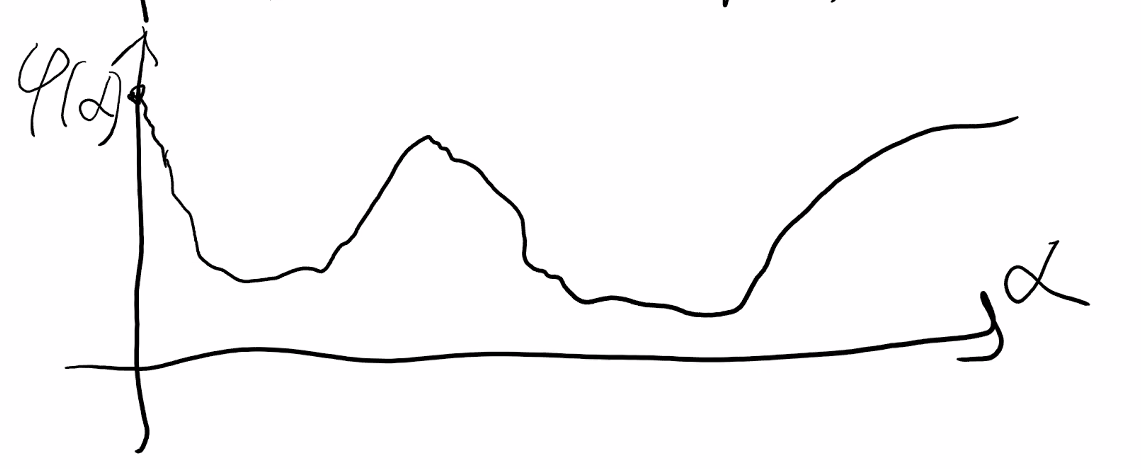
\includegraphics[scale=0.5]{img/methopt_one_dimensional_optimization_f_proect}
\end{center}

Наша задача~--- найти некоторый локальный минимум этой функции.

Встает два вопроса:
\begin{itemize}
    \item Как найти этот минимум?
    \item Как точно искать этот минимум?
\end{itemize}

Если вычислять очень точно, мы потратим очень много на это ресурсов.
Если искать не точно, есть риск потерять сходимость функции.

Какие бывают методы поиска локального минимума в этой задаче?

Пусть нам известна точка $x_k$, мы хотим найти еще две точки $x, y$, в одной из которых ($y$) функция будт меньше, а в другой ($z$), больше чем в той ($y$).

\begin{center}
    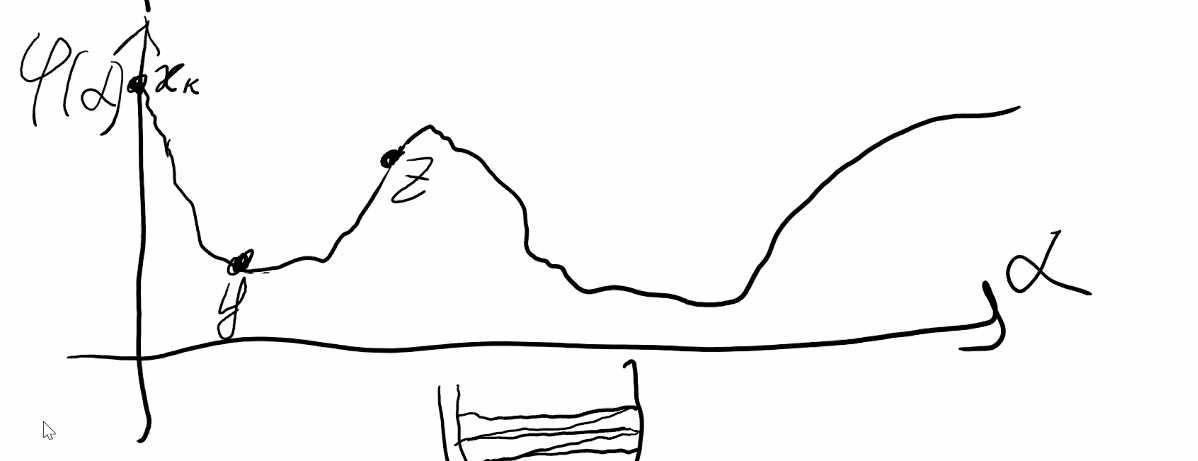
\includegraphics[scale=0.5]{img/methopt_one_dimensional_optimization_f_proect_points}
\end{center}

Как правило здесь используют довольно примитивные подходы.

У нас убывает функция, давайте возьмем некоторый шаг $\alpha$ (обчно $< 1$) и посчитаем $\varphi (\alpha)$.

Если там фунция меньше, чем $\varphi (0)$, то мы нашли $y$. Как найти $z$.
Давайте восколько-нибудь увеличим шаг $\alpha$, например, в два раза и посчитаем там $\varphi(2 \alpha)$.
Там может быть $\varphi(2 \alpha) > \varphi(\alpha)$, то $z = 2\alpha$.
Иначе, путь $y = 2\alpha$, а $z$ стоит попробовать найти еще раз.

Что делать, если $\varphi(\alpha) > \varphi(0)$.
Тогда возьмем $ \alpha / 2$ и попробуем сделать то же самое.

Допустим, мы нашли некоторый интервал, на котором есть минимум.
То есть есть три точки, в средней из которых функция меньше.
Один из способов дальшнейшего исслежования функции --- \textbf{метод дихатомии}.
Возьмем центр этого интервала и изучать поведение функции справа и слева от этой точки: $\varphi\left(\dfrac{a+b}{2} \pm h \right)$.
$h$ --- выбирается $\pm$ имперически.

\begin{center}
    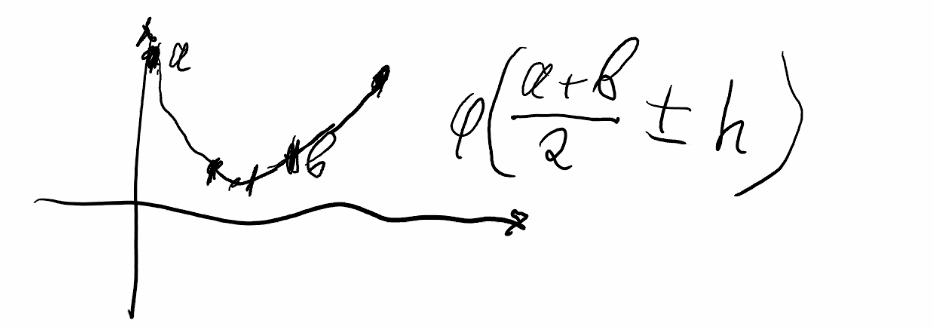
\includegraphics[scale=0.5]{img/methopt_one_dimensional_optimization_f_proect_pmh_points}
\end{center}

Дальше мы справниваем знаение функции слева и справа ($\pm h$) и переносим ближайшую крайнюю точку в точку с большим значением.
На рисунке выше мы перенесли $b$ в точку $\dfrac{a+b}{2}+h$.

Плюсы такого метода: простой метод (по модулю предположения, что функция унимодальна), считать просто.\\
Минусы: не очень сильно эффективен (на каждый шаг два вычисления функции).

Более эффективный метод: метод золотого сечения (метод Фибоначчи).

Еще один из простых, но при некоторых предположениях достаочно эффективный~--- \textbf{метод полиномиальной Аппроксимации}.
Предположим, что функция очень близка к какому-то полиному.
Самое просто~--- квадратичному полиному (параболе).

Пусть у нас есть три точки, проведем через них параболу.
Теперь аналичтически найдем точку минимума этой параболы и в этой точке посмотрим явное повдение нашей функции.

Дальше, так же, как в Дихатомии, сдвиним рассматриваемый отрезок фунции и повторим наши действия.

\begin{center}
    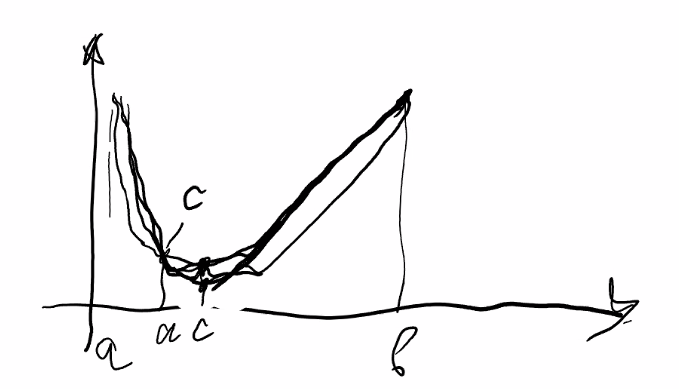
\includegraphics[scale=0.7]{img/methopt_one_dimensional_optimization_polynomial_approx}
\end{center}

Плюсы: если функция хорошая (достаточно гладкая, вблизи минимума хорошо аппроксимируется вблизи минимума).\\
Минусы: если функция плохая, будет работать очень не точно.

Еще можно аппроксимировать с использованием \textbf{производных}.
Пусть в точках $a$ и $b$ мы знаем не только значение $\varphi$, но и значение производной $\varphi^\prime$.

Для аппроксимации есть эрмитовы полиномы, их 4:
\begin{center}
    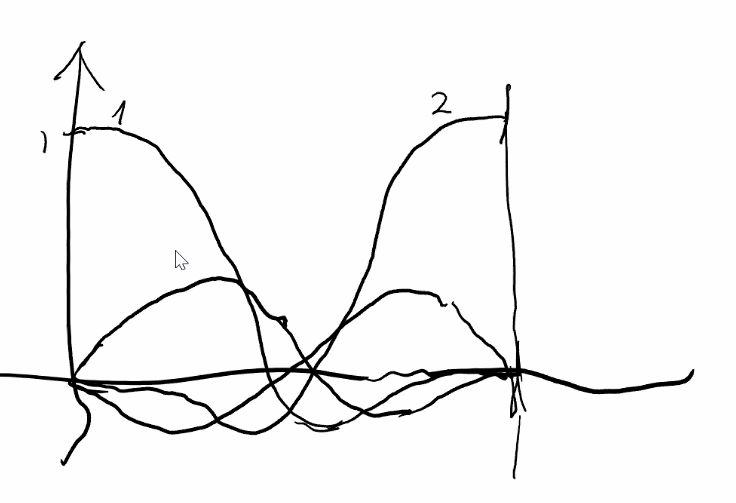
\includegraphics[scale=0.4]{img/methopt_one_dimensional_optimization_ermyt_polynom}
\end{center}

Возьмем:
$\varphi(a) E_1 + \varphi (b) E_2 + \varphi^\prime (a) E_3 + \varphi^\prime (b) E_4$.

Плюсы и минусы те же.
Кроме того, функция $\varphi$ должна быть достаточно гладкой, что бы мы могли вычисялять ее производные.

\textbf{Метод Ньютона} (метод касательных).
Строим касательные (производные), ищем их пересеченеи с нулем ($\varphi^\prime = 0$).
Найденные точки (нули) и есть ответ.

Плюсы: если функция квадратичная (или другая хорошая) будет очень быстро сходиться.\\
Минусы: нужны вторые производные.

\textbf{Метод секущих (хорд)}.
Так же, как в методе Ньютона, ищем нули.

\subsection{Условия Вольфе}

Условия выбора следующей точки для исследования ее на минимум.

\begin{itemize}
    \item $\varphi (\alpha) = f(x_k + \alpha p_k)$
    \item $f(x_k + \alpha p_k) \leqslant f(x_k) + c_1 \alpha \triangledown f (x_k) p_k$.\\
    $0 < c_1 < 1$, $c_1 = 10^{-4}$.
\end{itemize}

Первое условие накладывает вограничения на выбираемое $\alpha$.
\begin{center}
    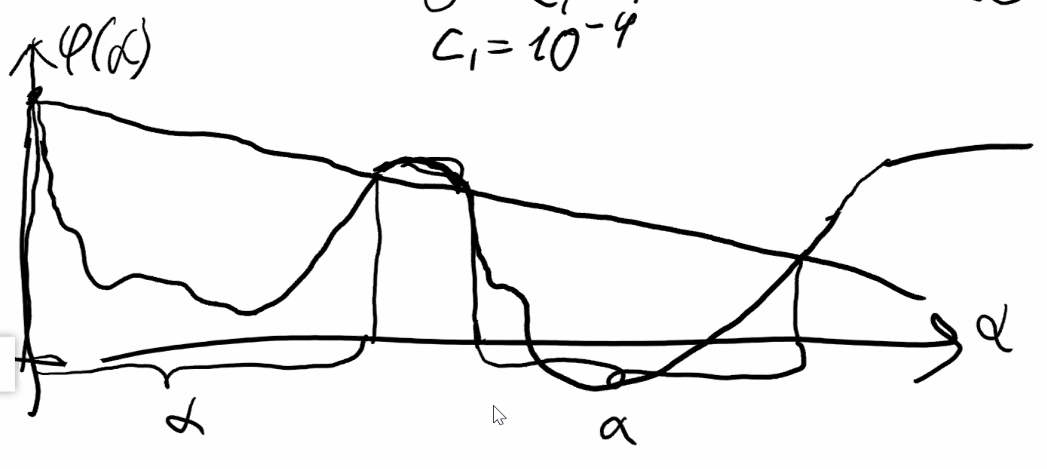
\includegraphics[scale=0.4]{img/methopt_volfe_conditions_1}
\end{center}

Первого условия не достаточно, так как можно взять $\alpha = \varepsilon$ и это условие там будет выполняться. \\
Второе условие заперщает делать делать слишком маленькие шаги и шагать туда, где градиент продолжает достаточно быстро убывать

\begin{center}
    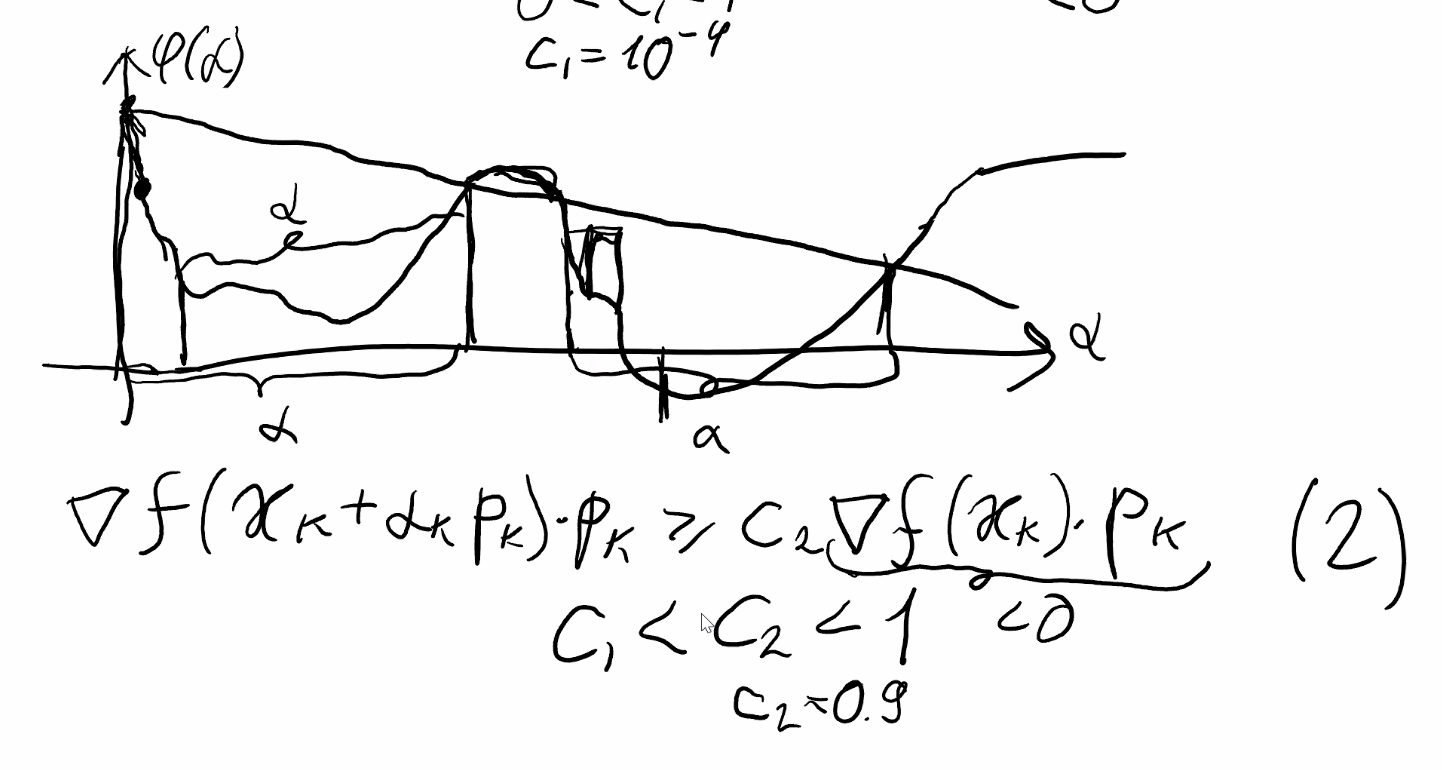
\includegraphics[scale=0.333]{img/methopt_volfe_conditions_2}
\end{center}

В целом, есть доказательство корректности условий Вольфа.
